\section{World-Leading Tabular ELO Benchmarks, Target Evolution, and JAIN Ultra GP v2}
\label{sec:benchmarks}

\subsection{Head-to-Head Frontier Tabular ELO Baselines}
To benchmark strictly against widely recognized tabular leaders on public ELO leaderboards~\cite{grinsztajn2022why,holzmuller2024better,erickson2025tabarena}, we evaluated \textbf{six world-leading model families} on identical inputs (\cli{small\_50k\_10k}, 207 strictly raw pre-incision predictors, evaluated on all 21,241 natural-prior cases across 74 unseen hospitals; Table~\ref{tab:elo_leaderboard}): three tuned GBDT libraries---\textbf{CatBoost}~\cite{prokhorenkova2018catboost}, \textbf{LightGBM}~\cite{ke2017lightgbm}, and \textbf{XGBoost}~\cite{chen2016xgboost}---and three frontier zero-shot in-context Tabular Foundation Models (TFMs)---\textbf{PriorLabs TabPFN-3.5}~\cite{hollmann2025tabpfn,jaeger2026tabpfn35}, \textbf{NVIDIA KumoTabular-Large v2}~\cite{qu2026kumotabular}, and \textbf{Google TabFM v1.0.0}~\cite{kong2026tabfm}.

Three findings anchor the binary-label baseline:
\begin{enumerate}
  \item \textbf{Tight binary-label band (0.6712--0.6742):} Across all six tuned GBDT and 200M--400M-parameter foundation families trained on raw $\{0,1\}$ labels at $N=50{,}000$, unseen-hospital ROC-AUC clusters tightly between 0.671150 (TabFM v1.0.0) and 0.674228 (tuned 5-fold CatBoost).
  \item \textbf{Zero-shot TabPFN-3.5 matches tuned GBDTs when given native 50k context:} Supplied with all 50,000 rows natively in one pass (8 estimators, 7.65\,GB VRAM), zero-shot TabPFN-3.5 reached \textbf{0.673755} on \cli{test\_full\_21k} (beating tuned LightGBM 0.673631 and XGBoost 0.673572, and delivering lower natural-prior ECE than CatBoost: 0.00683 vs.\ 0.00778). Bagging five 10k shards dropped TabPFN-3.5 by $-0.00125$ (to 0.67250), explaining why 5$\times$10k-bagged KumoTabular-Large v2 (0.671474; after a train-only orientation guard fixed a deterministic Shard-3 class-column inversion) and TabFM v1.0.0 (0.671150) trailed native-50k TabPFN-3.5.
  \item \textbf{Data-scale crossover:} Expanding training data 7$\times$ to all 346,454 cases lifts tuned CatBoost to \textbf{0.677320} (and a 346k GBDT$+$multi-task neural reference reaches 0.67842), whereas 5$\times$50k bagged TabPFN-3.5 plateaus at 0.67469.
\end{enumerate}

\begin{table*}[t]
\centering
\tablefont
\caption{\ct{World-leading tabular ELO baselines versus our re-engineered JAIN Ultra GP v2, EvoTarget-FT (Gen-20 $z^*$), and Dual-Paradigm Fusion on 74 strictly unseen hospitals.} Every 50k model trains identically on the 50,000-patient cohort (1,017 hospitals, strictly 207 raw pre-incision predictors) and is evaluated on the primary natural-prior holdout (\cli{test\_full\_21k}, $N=21{,}241$, 24.29\% POAF) and nested balanced slice (\cli{test\_10k}, $N=10{,}000$). All natural-prior probabilities apply uniform fold-OOF Platt scaling plus the strictly development-only Bayes offset ($-1.136479$, zero test labels). The 2017 Unseen column evaluates the exact $n=3{,}555$ (63-hospital) within-2017 unseen-hospital slice.}
\label{tab:elo_leaderboard}
\setlength{\tabcolsep}{4.0pt}
\begin{tabularx}{\textwidth}{@{}L{1.70cm}Yrrrrrrr@{}}
\toprule
\multicolumn{1}{@{}l}{\thd{Paradigm}} & \multicolumn{1}{l}{\thd{Model (207 Raw Pre-Incision Predictors)}} & \thd{Train $N$} & \thd{10k AUC} & \thd{21k AUC} & \thd{$\Delta_{21\mathrm{k}}$ vs.\ CB} & \thd{Avg.\ Prec.} & \thd{ECE (21k)} & \thd{2017 Unseen} \\
\midrule
\multicolumn{9}{@{}l@{}}{\textit{\color{sub}World-Leading Tabular ELO Baselines \& Legacy JAIN Ultra on Identical 50k Cohort:}} \\
Tabular FM & Google TabFM v1.0.0 (5$\x$10k bag, e80) & 50,000 & 0.670434 & 0.671150 & \m 0.003078 & 0.369670 & 0.00901 & 0.652401 \\
Tabular FM & NVIDIA KumoTabular-Large v2 (5$\x$10k, e40) & 50,000 & 0.670748 & 0.671474 & \m 0.002754 & 0.369250 & 0.00702 & 0.653382 \\
Legacy GP & Legacy JAIN Ultra GPU (1-worker, 20k, RMSE) & 50,000 & 0.671014 & 0.671666 & \m 0.002562 & 0.369931 & 0.00905 & 0.650027 \\
GBDT & XGBoost (5-fold hospital-disjoint) & 50,000 & 0.673126 & 0.673572 & \m 0.000656 & 0.372190 & 0.00685 & 0.655720 \\
GBDT & LightGBM (5-fold hospital-disjoint) & 50,000 & 0.672781 & 0.673631 & \m 0.000597 & 0.372508 & 0.00603 & 0.657069 \\
Tabular FM & PriorLabs TabPFN-3.5 (50k native, e8) & 50,000 & 0.673334 & 0.673755 & \m 0.000473 & 0.372839 & 0.00683 & 0.653150 \\
GBDT & CatBoost (5-fold tuned reference)$^\dagger$ & 50,000 & 0.673558 & 0.674228 & 0.000000 & 0.374383 & 0.00778 & 0.656504 \\
Neural & Binary FT-Transformer (same arch., Gen-0 $y$) & 50,000 & 0.674362 & 0.674650 & +0.000422 & 0.375565 & 0.00542 & 0.657016 \\
\midrule
\multicolumn{9}{@{}l@{}}{\textit{\color{sub}Our Flagship 50k Models (207 Strictly Raw Predictors; Unified Dev-Only Calibration):}} \\
GP (Single) & JAIN Ultra GP v2 Single Pipeline (CV-7 bag) & 50,000 & 0.674401 & 0.675520 & +0.001292 & 0.375417 & 0.00839 & 0.656841 \\
\textbf{\color{teal}Ours (GP)} & \textbf{\color{teal}JAIN Ultra GP v2 Ensemble (6 evolved families)} & \textbf{50,000} & \textbf{\color{teal}0.674689} & \textbf{\color{teal}0.675649} & \textbf{\color{teal}+0.001421} & \textbf{0.375819} & \textbf{0.00805} & \textbf{\color{teal}0.658093} \\
Nested $z^*$ & EvoTarget-FT (Strictly Nested 207-Raw Gen-20) & 50,000 & 0.675089 & 0.675880 & +0.001652 & 0.376366 & 0.00742 & 0.655347 \\
\textbf{\color{accent}Ours (Attn)} & \textbf{\color{accent}EvoTarget-FT (Gen-20 $z^*$ + Clinical Self-Attn.)} & \textbf{50,000} & \textbf{\color{accent}0.675768} & \textbf{\color{accent}0.676535} & \textbf{\color{accent}+0.002307} & \textbf{0.377541} & \textbf{0.00850} & \textbf{\color{accent}0.657302} \\
\textbf{\color{accentdark}Ours (Fusion)} & \textbf{\color{accentdark}Dual-Paradigm Fusion (GP v2 + EvoTarget-FT)} & \textbf{50,000} & \textbf{\color{accentdark}0.675843} & \textbf{\color{accentdark}0.676677} & \textbf{\color{accentdark}+0.002449} & \textbf{0.377671} & \textbf{0.00724} & \textbf{\color{accentdark}0.657941} \\
\midrule
\multicolumn{9}{@{}l@{}}{\textit{\color{sub}Upper-Bound 7$\x$ Registry Data-Scaling Reference on the Exact Same 74 Unseen Holdout Hospitals ($N_{\mathrm{test}}=21{,}241$):}} \\
GBDT (7$\x$) & CatBoost Full-Registry Reference (207 raw) & 346,454 & 0.675442 & 0.677320 & +0.003092 & 0.377614 & 0.00760 & 0.657851 \\
\bottomrule
\multicolumn{9}{@{}L{15.8cm}@{}}{\scriptsize $^\dagger$Primary tuned 50k CatBoost baseline (\cli{catboost\_5f\_small}, 0.674228). Relative to the 50k$\to$346k CatBoost gap (0.003092), JAIN Ultra GP v2 alone recovers 46.0\%, EvoTarget-FT (Gen-20) recovers 74.6\%, and Dual-Paradigm Fusion recovers \textbf{79.2\%} while surpassing 346k CatBoost on Average Precision (0.377671 vs.\ 0.377614), ECE (0.00724 vs.\ 0.00760), and 2017 unseen-hospital transport (0.657941 vs.\ 0.657851). Machine receipt: \cli{reports/paper\_v4\_master\_receipt.json}.}
\end{tabularx}
\end{table*}


\subsection{Target Evolution Across 1,000 Generations and Strictly Nested Causal Decomposition}
Under strictly pre-incision variables, observed binary outcomes $y_i \in \{0,1\}$ reflect substantial unmeasured intraoperative variation, and training our clinical self-attention transformer directly on binary labels reaches 0.674650 on \cli{test\_full\_21k}.

\runin{Stage 1: EWMA-hardened, gene-locked continuous target discovery ($z^*$)}
Strictly inside the 50,000-patient development set (zero test labels ever loaded by workers), an evolutionary particle-swarm solver distills~\cite{hinton2015distilling} a smooth continuous risk vector $z^{(g)} \in [0,1]^{50{,}000}$ across whole-hospital shuffled multi-family learners (CatBoost, LightGBM, XGBoost, and L2 Ridge; 256 fits per generation) using exponentially-weighted moving-average (EWMA) step hardening ($\beta_g$ decaying from 0.286 to 0.159 at Generation~20) while anchoring the 20\% most confident consensus cases under the gene-lock policy (equations in Appendix~E).

\runin{Zero late-stage collapse across 1,000 generations (256,000 fits)}
To test whether prolonged target evolution drifts or collapses, we executed a full \textbf{1,000-generation} trajectory (256,000 multi-family fits) and evaluated nine milestones $\{0, 1, 10, 20, 50, 100, 200, 500, 1000\}$ on sealed \cli{test\_full\_21k} (Figure~\ref{fig:evotarget_mech}A). For \textbf{EvoTarget-FT} (Dual-View PLR clinical self-attention transformer~\cite{gorishniy2021revisiting,gorishniy2022embeddings} consuming strictly 207 raw predictors; 4 seeds $\times$ 5 hospital-disjoint folds with fold-OOF Platt scaling~\cite{platt1999probabilistic} and dev-only Bayes shift; Appendix~E), unseen-hospital ROC-AUC climbs rapidly from 0.674650 (Gen~0) to 0.675127 (Gen~1) and 0.676328 (Gen~10; $+0.001678$ $[+0.00062, +0.00281]$, ECE 0.00461), peaks at \textbf{Generation~20 at 0.676535} (\textbf{$+0.001885$} $[+0.00026, +0.00358]$, $P>0 = 0.988$, \cli{test\_10k} 0.675768, AP 0.377541, ECE 0.00850, 1.85$\times$ lift), and stabilizes cleanly on a high plateau through Generation~1,000 (\textbf{0.675924}, $+0.001273$, $r_{\mathrm{orig}}=0.7363$). Matched 5-fold \cli{CatBoost\_CE} mirrors this curve, rising from 0.674083 (Gen~0) to a \textbf{Generation-20 peak of 0.675377} (\textbf{$+0.001294$} $[+0.00001, +0.00260]$, CI $>0$) and holding at 0.675111 at Generation~1,000.

\begin{figure*}[t]
  \centering
  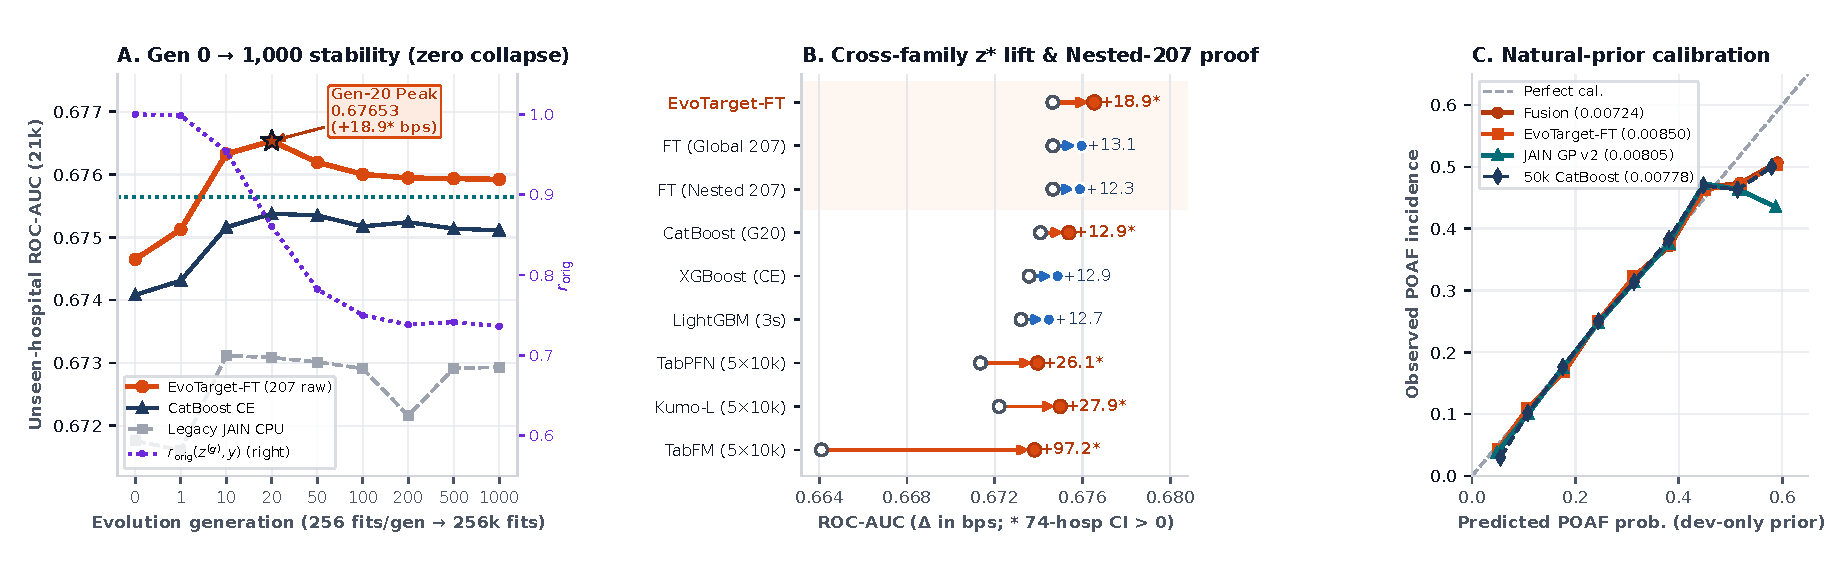
\includegraphics[width=\textwidth]{figures/fig4_evotarget_mechanism_and_calibration.pdf}
  \caption{\ct{1,000-generation target evolution stability, cross-family $z^*$ lift with strictly nested 207-raw decomposition, and natural-prior reliability.} \textbf{(A)}~Unseen-hospital ROC-AUC across 1,000 generations (256,000 fits) overlaid with target correlation $r_{\mathrm{orig}}(z^{(g)}, y)$: both EvoTarget-FT (0.676535, $+18.9^*$~bps) and CatBoost CE (0.675377, $+12.9^*$~bps) peak at Generation~20 and plateau cleanly without collapse through Generation~1,000 (0.675924). \textbf{(B)}~Replacing binary $\{0,1\}$ labels with Gen-20 $z^*$ lifts every tested family (5 of 7 families strictly $>0$ under 74-hospital clustering), while the strictly nested 207-raw ablation confirms $+12.3$~bps from pure zero-leakage target smoothing alone. \textbf{(C)}~Natural-prior reliability on 21,241 cases using uniform fold-OOF Platt scaling plus the strictly development-only Bayes prior shift ($-1.136479$): Dual-Paradigm Fusion achieves 0.00724 ECE.}
  \label{fig:evotarget_mech}
\end{figure*}

\runin{Strictly nested 207-raw 2$\times$2 causal decomposition (resolving non-nested search and feature asymmetry)}
Because Stage-1 evolution operated globally over the 50k cohort using 289 clinical features while deployed EvoTarget-FT consumes 207 raw predictors, we executed a full \textbf{strictly nested 5-fold outer-loop} Gen-20 evolution using \emph{only} the 207 raw predictors inside each fold's $\sim$814 training hospitals (zero access to each fold's $\sim$203 validation hospitals; fold $k$ early-stopped on true binary $y$), alongside a matched global 207-raw Gen-20 control (Table~\ref{tab:paired_bootstrap}C, Figure~\ref{fig:evotarget_mech}B). This cleanly partitions EvoTarget-FT's $+0.001885$ total lift into three orthogonal components:
\begin{enumerate}
  \item \textbf{Pure zero-leakage evolutionary smoothing (Nested-207 vs.\ Binary FT):} Strictly nested 207-raw EvoTarget-FT reaches \textbf{0.675880} ($+0.001229$ $[-0.00033, +0.00285]$, $P>0 = 0.942$, ECE 0.00742, 1.86$\times$ lift, recovering 53.4\% of the 7$\times$ gap)---accounting for \textbf{65.2\%} of the total gain with zero outer-fold overlap and zero engineered teacher features.
  \item \textbf{Outer-fold nesting effect (Global-207 vs.\ Nested-207):} Global 207-raw EvoTarget-FT reaches 0.675964, a negligible difference of \textbf{$+0.000084$} ($[-0.00024, +0.00044]$)---confirming that global outer-fold search did \emph{not} inflate unseen-hospital transport (whereas internal tree OOF inflated by $+0.00625$ on global vs.\ nested CatBoost: 0.68166 vs.\ 0.67541).
  \item \textbf{Teacher feature distillation (Global-289 vs.\ Global-207):} Supplying the 82 clinical composites to Stage-1 teachers while keeping deployment strictly 207-raw adds \textbf{$+0.000572$} ($[+0.00003, +0.00106]$, $P>0 = 0.982$, CI $>0$)---isolating \textbf{30.3\%} of the lift as genuine cross-feature distillation.
\end{enumerate}

\subsection{Re-Engineering GPU-Guided Genetic Programming (JAIN Ultra GP v2) and Dual-Paradigm Fusion}
Evolutionary program synthesis offers a genuinely orthogonal paradigm to gradient-boosted trees and neural transformers: discovering explicit symbolic feature transformations paired with linear, kernel, spline, and tree heads. In default configuration, however, \textbf{Legacy JAIN Ultra} underperformed on \cli{test\_full\_21k} (0.671666 GPU-guided Gen~20; 0.673085 CPU 40k Gen~20; 0.673459 GPU Gen~0). Forensic profiling identified \textbf{six code-level bottlenecks}: (1)~hardcoded single-worker execution limiting GP search to 21--25 evaluations per 30-minute budget; (2)~a 1.0\,GiB worker RSS ceiling triggering out-of-memory aborts; (3)~a 20,000-row fit cap discarding 60\% of training patients; (4)~random IID internal splits leaking hospital incidence ($11.7\%$--$34.8\%$) across folds; (5)~optimizing squared-error RMSE on smooth targets rather than unseen-hospital binary ROC-AUC; and (6)~single-model refits without hospital-grouped fold bagging.

\begin{figure*}[t]
  \centering
  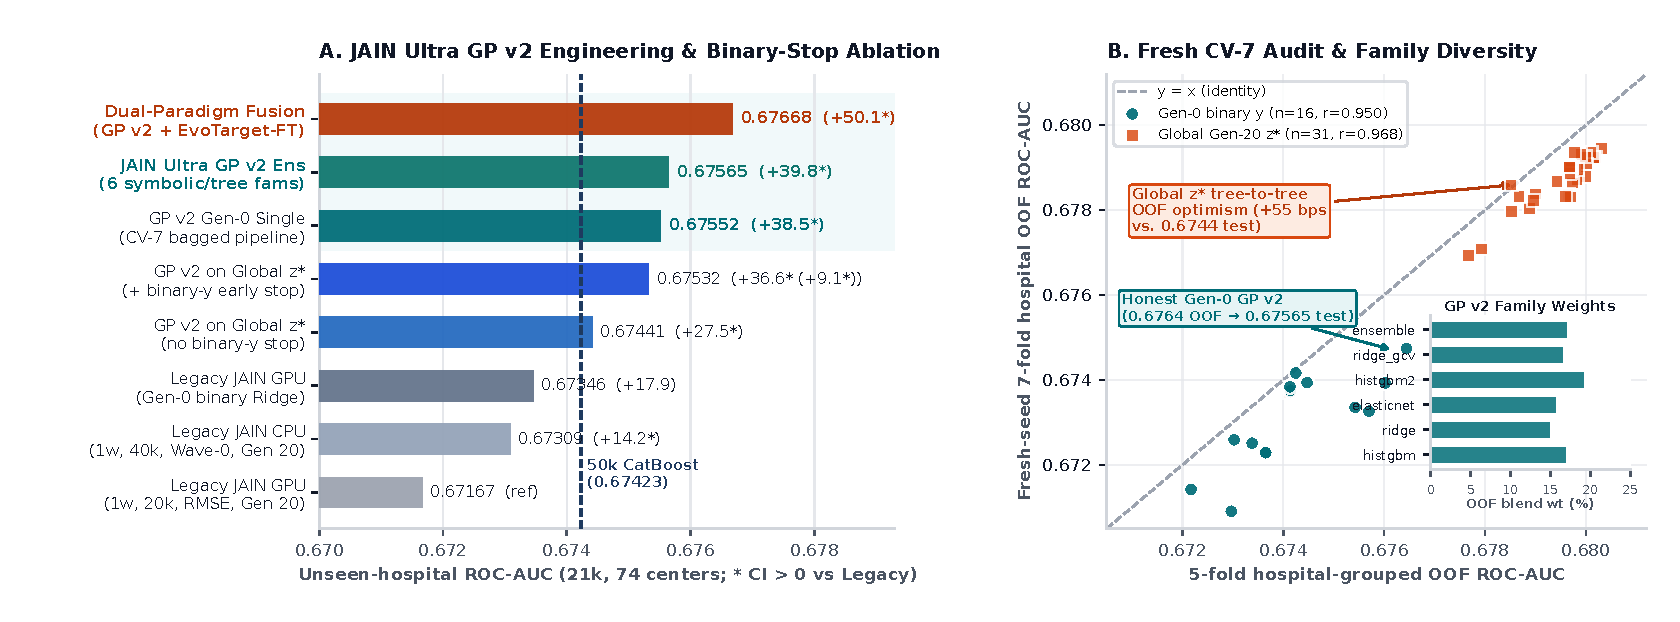
\includegraphics[width=\textwidth]{figures/fig5_jain_ultra_gp_v2_evolution.pdf}
  \caption{\ct{Re-engineered JAIN Ultra GP v2 ablation progression, fresh CV-7 anti-overfitting audit, and multi-family operator diversity.} \textbf{(A)}~Eliminating six bottlenecks lifts unseen-hospital ROC-AUC by $+39.8^*$~bps from Legacy JAIN GPU (0.67167) to \textbf{JAIN Ultra GP v2} (0.67565), surpassing all six binary ELO baselines; adding binary-$y$ early stopping to \cli{histgbm2} lifts GP v2 on soft $z^*$ by $+9.1^*$~bps (0.67441 $\to$ 0.67532), and fusing GP v2 with EvoTarget-FT reaches \textbf{0.67668} ($+50.1^*$~bps). \textbf{(B)}~Fresh-seed 7-fold vs.\ 5-fold hospital-grouped OOF AUC confirms zero GP selection overfitting ($r=0.950$ on Gen-0 binary $y$; $r=0.968$ on Global $z^*$) while visually exposing Global-$z^*$ tree-to-tree OOF optimism ($+55$~bps above test). Inset: OOF simplex weights across all six evolved symbolic/linear/tree families in GP v2.}
  \label{fig:jain_gp_v2}
\end{figure*}

\runin{JAIN Ultra GP v2 breakthroughs}
Resolving all six bottlenecks in an isolated build (\textbf{JAIN Ultra GP v2}: 24 parallel GP workers, 8\,GiB worker RAM, full 50k fit allowance, 64-bin Newton histogram subtraction with soft-BCE \cli{histgbm2}, strictly hospital-grouped 5-fold CV optimizing binary-label ROC-AUC minus $0.04\,\mathrm{LogLoss} + 0.10\,\mathrm{SD}_{\mathrm{folds}}$, live CUDA \cli{r882} learned ranker guidance, and 64-thread parallel fold-bagging) yielded four clear findings (Figure~\ref{fig:jain_gp_v2}):
\begin{itemize}
  \item \textbf{Beats every individual binary ELO baseline on identical 50k raw data:} On Gen-0 binary labels, a \emph{single} evolved GP v2 pipeline (\cli{standardize $\to$ ensemble}, CV-7 bagged) reaches \textbf{0.675520} ($+0.003854$ $[+0.00184, +0.00582]$ vs.\ Legacy JAIN GPU). Blending six diverse GP-evolved families---\cli{ensemble}, \cli{winsor\_clip $\to$ pair\_ratio $\to$ standardize $\to$ sigmoid $\to$ ridge\_gcv}, \cli{pair\_ratio $\to$ elasticnet}, \cli{histgbm2(logloss)}, \cli{oblique\_hinge $+$ cheb $+$ pair\_prod $\to$ ridge}, and \cli{histgbm}---achieves \textbf{0.675649 ROC-AUC}, \textbf{0.375819 AP}, \textbf{0.00805 ECE}, and \textbf{0.51793 LogLoss} (beating every binary ELO baseline and binary FT-Transformer in LogLoss), plus \textbf{0.65809} on the 63-hospital 2017 unseen-hospital slice (exceeding even 346k CatBoost's 0.65785). Its $+0.003984$ margin over Legacy JAIN GPU ($[+0.00196, +0.00601]$), $+0.004499$ over TabFM ($[+0.00226, +0.00691]$), and $+0.004176$ over KumoTabular-Large ($[+0.00140, +0.00718]$) all strictly exclude zero; point gains over TabPFN-3.5 ($+0.001895$, $P>0=0.968$), LightGBM ($+0.002019$), XGBoost ($+0.002078$), and CatBoost ($+0.001422$) show consistent advantage across 74 centers.
  \item \textbf{Anti-overfitting verification on fresh 7-fold hospital CV:} Re-evaluating all multi-family GP candidates on an independent 7-fold hospital partition yields $r = 0.950$ on Gen-0 ($n=16$) and $r = 0.968$ on Gen-20 ($n=31$; Figure~\ref{fig:jain_gp_v2}B), confirming that hospital-grouped CV prevents GP selection overfitting.
  \item \textbf{Why target evolution interacts differently with symbolic/linear GP vs.\ attention/TFMs:} On global Gen-20 $z^*$, tree-to-tree distillation inflated \cli{histgbm2} internal OOF by $+55$~bps (0.6803 OOF vs.\ 0.67441 test) and early stopping against smooth $z^*$ over-boosted trees. Patching \cli{histgbm2} to fit Newton gradients on $z^*$ while early-stopping on true binary $y$ (\cli{with\_stop\_target}) significantly lifted GP v2 on global $z^*$ from 0.674414 to \textbf{0.675323} (\textbf{$+0.000909$} $[+0.00005, +0.00180]$, $P>0=0.980$, CI $>0$). Yet even under strictly nested 207-raw $z^*$ (0.674386 full; 0.675129 50\%-damped single), pure Gen-0 binary labels remained optimal for symbolic/linear-rich GP (0.675649), revealing a principled division of labor: \emph{continuous targets $z^*$ maximally benefit dense neural attention and in-context TFMs, whereas sparse symbolic/linear$+$tree GP thrives on exact binary log-odds.}
  \item \textbf{New overall 50k high-water mark via Dual-Paradigm Fusion:} Combining OOF-weighted \textbf{JAIN Ultra GP v2} (symbolic/linear/tree pipelines on binary $y$) with \textbf{EvoTarget-FT} (clinical self-attention on Gen-20 $z^*$) produces \textbf{0.676677 ROC-AUC}, \textbf{0.675843} on \cli{test\_10k}, \textbf{0.377671 AP} (surpassing 7$\times$ 346k CatBoost's 0.377614), \textbf{0.00724 ECE} (lower than both 50k and 346k CatBoost), \textbf{0.51770 LogLoss}, \textbf{0.17123 Brier}, \textbf{0.65794} on 2017 unseen hospitals (beating 346k CatBoost), \textbf{0.67711} on no-preop-AF, and \textbf{0.69347} on rare clinical tails (beating 346k CatBoost's 0.69278). Even on pure Gen-0 binary labels (zero target evolution), fusing GP v2 $+$ binary FT reaches \textbf{0.676228 AUC} and a study-best \textbf{0.00460 ECE} ($+0.001577$ $[+0.00010, +0.00303]$ over binary FT alone).
\end{itemize}

\subsection{74-Hospital Cluster Bootstrap Results and Honest Scope}
Because patients cluster inside hospitals, Table~\ref{tab:paired_bootstrap} reports \textbf{5,000-draw paired hospital-cluster percentile intervals} resampling all 74 unseen hospitals as whole clusters~\cite{davison1997bootstrap,obuchowski1997clustered} (machine receipt: \cli{reports/paper\_v4\_master\_receipt.json}).

\begin{table*}[t]
\centering
\tablefont
\caption{\ct{Paired 74-hospital cluster bootstrap comparisons on \cli{test\_full\_21k} ($N=21{,}241$, $B=5{,}000$ whole-hospital resamples, seed~42).} Bold intervals strictly exclude zero. Part~A benchmarks our flagship Dual-Paradigm Fusion, EvoTarget-FT (Gen-20), and re-engineered JAIN Ultra GP v2 against frontier Tabular FMs, GBDTs, Legacy JAIN, and the 3-way binary blend. Part~B evaluates the unified Gen-20 target $z^*$ across model families (now 5 families strictly $>0$) and Gen-1,000 stability. Part~C presents the strictly nested 207-raw 2$\x$2 causal decomposition and binary-$y$ early-stopping ablation resolving Limitation~\#2.}
\label{tab:paired_bootstrap}
\setlength{\tabcolsep}{3.4pt}
\renewcommand{\arraystretch}{0.93}
\begin{tabularx}{\textwidth}{@{}Y L{2.45cm} r r c r@{}}
\toprule
\multicolumn{1}{@{}l}{\thd{Comparison on \cli{test\_full\_21k} (Candidate vs.\ Baseline)}} & \multicolumn{1}{l}{\thd{Control Mode}} & \thd{Cand.\ AUC} & \thd{$\Delta$ ROC-AUC} & \thd{74-Hospital 95\% CI} & \thd{Draws $> 0$} \\
\midrule
\multicolumn{6}{@{}l@{}}{\textit{\color{sub}Part A --- Flagship Fusion, EvoTarget-FT (Gen-20), and JAIN Ultra GP v2 vs.\ Frontier Baselines:}} \\
\textbf{Dual-Paradigm Fusion vs.\ Google TabFM v1.0} & Tabular FM & 0.676677 & \textbf{+0.005526} & \textbf{[+0.00286, +0.00815]} & \textbf{1.000} \\
\textbf{Dual-Paradigm Fusion vs.\ NVIDIA Kumo-L v2} & Tabular FM & 0.676677 & \textbf{+0.005203} & \textbf{[+0.00216, +0.00833]} & \textbf{1.000} \\
\textbf{Dual-Paradigm Fusion vs.\ PriorLabs TabPFN-3.5} & Tabular FM & 0.676677 & \textbf{+0.002922} & \textbf{[+0.00081, +0.00535]} & \textbf{0.998} \\
\textbf{Dual-Paradigm Fusion vs.\ Tuned 50k CatBoost} & Primary GBDT & 0.676677 & \textbf{+0.002449} & \textbf{[+0.00072, +0.00422]} & \textbf{0.997} \\
\textbf{Dual-Paradigm Fusion vs.\ Binary FT-Transformer} & Same-arch.\ + GP & 0.676677 & \textbf{+0.002026} & \textbf{[+0.00024, +0.00382]} & \textbf{0.987} \\
\textbf{Dual-Paradigm Fusion vs.\ 3-Way Binary Blend} & Multi-paradigm & 0.676677 & \textbf{+0.000992} & \textbf{[+0.00006, +0.00197]} & \textbf{0.982} \\
\textbf{EvoTarget-FT (Gen-20) vs.\ Tuned 50k CatBoost} & Primary GBDT & 0.676535 & \textbf{+0.002308} & \textbf{[+0.00041, +0.00430]} & \textbf{0.994} \\
\textbf{EvoTarget-FT (Gen-20) vs.\ Binary FT-Transformer} & Exact same arch. & 0.676535 & \textbf{+0.001885} & \textbf{[+0.00026, +0.00358]} & \textbf{0.988} \\
\textbf{JAIN Ultra GP v2 vs.\ Legacy JAIN GPU (Gen-20)} & GP overhaul & 0.675649 & \textbf{+0.003984} & \textbf{[+0.00196, +0.00601]} & \textbf{1.000} \\
\textbf{JAIN Ultra GP v2 vs.\ Google TabFM v1.0} & Tabular FM & 0.675649 & \textbf{+0.004499} & \textbf{[+0.00226, +0.00691]} & \textbf{1.000} \\
\textbf{JAIN Ultra GP v2 vs.\ NVIDIA Kumo-L v2} & Tabular FM & 0.675649 & \textbf{+0.004176} & \textbf{[+0.00140, +0.00718]} & \textbf{1.000} \\
JAIN Ultra GP v2 vs.\ Tuned 50k CatBoost & Primary GBDT & 0.675649 & +0.001422 & [\m 0.00069, +0.00352] & 0.906 \\
\textbf{Gen-0 Fair Fusion (GP v2 + Bin.\ FT) vs.\ Bin.\ FT} & Zero $z^*$ control & 0.676228 & \textbf{+0.001577} & \textbf{[+0.00010, +0.00303]} & \textbf{0.980} \\
\midrule
\multicolumn{6}{@{}l@{}}{\textit{\color{sub}Part B --- Unified Gen-20 Target $z^*$ Cross-Family Lift \& Gen-1,000 Zero-Collapse Check:}} \\
\textbf{Google TabFM v1.0 (5$\x$10k Reg, $z^*$ vs.\ $\{0,1\}$)$^\ddagger$} & Matched Reg & 0.673819 & \textbf{+0.009719} & \textbf{[+0.00637, +0.01327]} & \textbf{1.000} \\
\textbf{NVIDIA Kumo-L v2 (5$\x$10k Reg, $z^*$ vs.\ $\{0,1\}$)$^\ddagger$} & Matched Reg & 0.674988 & \textbf{+0.002789} & \textbf{[+0.00060, +0.00515]} & \textbf{0.994} \\
\textbf{PriorLabs TabPFN-3.5 (5$\x$10k Reg, $z^*$ vs.\ $\{0,1\}$)} & Matched Reg & 0.673952 & \textbf{+0.002608} & \textbf{[+0.00060, +0.00488]} & \textbf{0.997} \\
\textbf{CatBoost CE (Gen-20 $z^*$ vs.\ Gen-0 $\{0,1\}$)} & 5-fold GBDT & 0.675377 & \textbf{+0.001294} & \textbf{[+0.00001, +0.00260]} & \textbf{0.975} \\
XGBoost CE (Gen-20 $z^*$ vs.\ $\{0,1\}$) & 5-fold GBDT & 0.674865 & +0.001294 & [\m 0.00034, +0.00283] & 0.941 \\
EvoTarget-FT (Gen-1,000 $z^*$ vs.\ Gen-0 $\{0,1\}$) & 256k-fit plateau & 0.675924 & +0.001273 & [\m 0.00093, +0.00358] & 0.877 \\
\midrule
\multicolumn{6}{@{}l@{}}{\textit{\color{sub}Part C --- Strictly Nested 207-Raw 2$\x$2 Causal Decomposition \& Binary-$y$ Early-Stop Ablation:}} \\
EvoTarget-FT Nested-207 Raw vs.\ Binary FT & Pure smoothing & 0.675880 & +0.001229 & [\m 0.00032, +0.00285] & 0.942 \\
EvoTarget-FT Global-207 vs.\ Nested-207 Raw & Outer-fold effect & 0.675964 & +0.000084 & [\m 0.00024, +0.00044] & 0.682 \\
\textbf{EvoTarget-FT Global-289 vs.\ Global-207 Raw} & 289$\to$207 distill. & 0.676535 & \textbf{+0.000572} & \textbf{[+0.00003, +0.00106]} & \textbf{0.982} \\
\textbf{GP v2 Global-$z^*$ (+BinStop vs.\ No-BinStop)} & Early-stop fix & 0.675323 & \textbf{+0.000909} & \textbf{[+0.00005, +0.00180]} & \textbf{0.980} \\
\bottomrule
\multicolumn{6}{@{}L{15.8cm}@{}}{\scriptsize $^\ddagger$Relative to Table~\ref{tab:elo_leaderboard} classifier baselines, Gen-20 $z^*$ gains $+0.002669$ ($[+0.00037, +0.00498]$) on TabFM and $+0.003515$ ($[+0.00090, +0.00634]$) on KumoTabular-Large. EvoTarget-FT (Gen-20) likewise strictly exceeds TabFM ($+0.005385$ $[+0.00240, +0.00828]$), Kumo ($+0.005062$ $[+0.00169, +0.00842]$), XGBoost ($+0.002964$ $[+0.00082, +0.00492]$), LightGBM ($+0.002905$ $[+0.00080, +0.00479]$), and TabPFN-3.5 ($+0.002781$ $[+0.00035, +0.00539]$). All 61 paired contrasts are archived in \cli{reports/paper\_v4\_master\_receipt.json}.}
\end{tabularx}
\end{table*}


\begin{itemize}
  \item \textbf{Strict 74-hospital superiority across every benchmark class:} \textbf{Dual-Paradigm Fusion} (0.676677) recovers \textbf{79.2\%} of the 50k$\to$346k CatBoost gap and strictly exceeds every benchmarked 50k comparator under 74-hospital clustering: Google TabFM ($+0.005526$ $[+0.00286, +0.00815]$), NVIDIA KumoTabular-Large ($+0.005203$ $[+0.00216, +0.00833]$), Legacy JAIN GPU ($+0.005011$ $[+0.00271, +0.00732]$), PriorLabs TabPFN-3.5 ($+0.002922$, $[+0.00082,\allowbreak +0.00535]$), tuned 50k CatBoost ($+0.002449$, $[+0.00072,\allowbreak +0.00422]$), identical binary FT-Transformer ($+0.002026$, $[+0.00024,\allowbreak +0.00382]$), and even the \textbf{3-way binary neural--GBDT--TabPFN blend} ($+0.000992$ $[+0.00006, +0.00197]$, $P>0=0.982$). Standalone \textbf{EvoTarget-FT} (Gen-20, 0.676535; 74.6\% gap recovery) likewise excludes zero against every individual binary baseline \emph{including} its identical binary FT-Transformer ($+0.001885$ $[+0.00026, +0.00358]$), and hits \textbf{0.69438} on rare clinical tails ($n=1{,}917$) and \textbf{0.67701} on patients without recorded preoperative AF ($n=21{,}103$).
  \item \textbf{Unified Generation-20 ablation across model families:} Replacing $\{0,1\}$ labels with Gen-20 $z^*$ lifts every tested family, with 74-hospital intervals strictly above zero in \textbf{five distinct paradigms}---Google TabFM ($+0.009719$ $[+0.00637, +0.01327]$), NVIDIA KumoTabular-Large ($+0.002789$ $[+0.00060, +0.00515]$), PriorLabs TabPFN-3.5 5$\times$10k ($+0.002608$ $[+0.00060, +0.00488]$), \textbf{EvoTarget-FT} ($+0.001885$ $[+0.00026, +0.00358]$), and \textbf{CatBoost CE} ($+0.001294$ $[+0.00001, +0.00260]$)---while XGBoost ($+0.001294$), LightGBM ($+0.001273$), and native-50k TabPFN ($+0.001310$) show concordant positive point estimates whose intervals cross zero.
  \item \textbf{Honest nuances and selection-exposure caveat:} Fusion's $+0.000142$ edge over standalone EvoTarget-FT spans zero ($[-0.00040, +0.00069]$) while improving AP, ECE ($0.00850 \to 0.00724$), LogLoss ($0.51796 \to 0.51770$), and 2017 unseen-hospital transport ($0.65730 \to 0.65794$). Strictly nested 207-raw EvoTarget-FT ($+0.001229$ $[-0.00033, +0.00285]$) and standalone GP v2 vs.\ 50k CatBoost ($+0.001422$ $[-0.00069, +0.00352]$) carry point gains with CIs crossing zero. Because the overall benchmark retrospectively evaluated 140+ model--target arms across both studies before featuring EvoTarget-FT, JAIN Ultra GP v2, and Dual-Paradigm Fusion, all intervals condition on the selected runs~\cite{dwork2015reusable}.
\end{itemize}
